% Generado por sistema/backend ReporteTex.java -- no editar a mano.
% Datos: /private/tmp/claude-501/-Users-miguel-project-taller-s/a868368b-4351-4d87-8017-fb9a5bc093aa/scratchpad/titulados.csv (titulados) / /private/tmp/claude-501/-Users-miguel-project-taller-s/a868368b-4351-4d87-8017-fb9a5bc093aa/scratchpad/empleadores.csv (empleadores)
De los 14 cruces de la Sección~\ref{sec:cruces}, 6 muestran dependencia significativa: ahí una variable incide directamente sobre la otra.

\begin{mitabla}{Cruces con dependencia significativa ($\alpha = 0.05$)}
\begin{tabular}{clcc}
\toprule
Id & $X$ incide sobre $Y$ & $X_0^2$ & $X_{0.05,\,gl}^2$ \\
\midrule
C7 & Nivel cursado incide sobre Financiamiento & 4.53 & 3.84 \\
C8 & Edad incide sobre Área de interés & 20.77 & 9.49 \\
C9 & Experiencia incide sobre Remuneración & 32.08 & 3.84 \\
C10 & Experiencia incide sobre Cargo & 4.71 & 3.84 \\
C11 & Formación complementaria incide sobre Interés en posgrado & 4.46 & 3.84 \\
C12 & Edad incide sobre Situación laboral & 22.43 & 9.49 \\
\bottomrule
\end{tabular}
\end{mitabla}

\begin{figure}[H]
\centering
\caption{$X_0^2$ de los cruces con dependencia significativa}
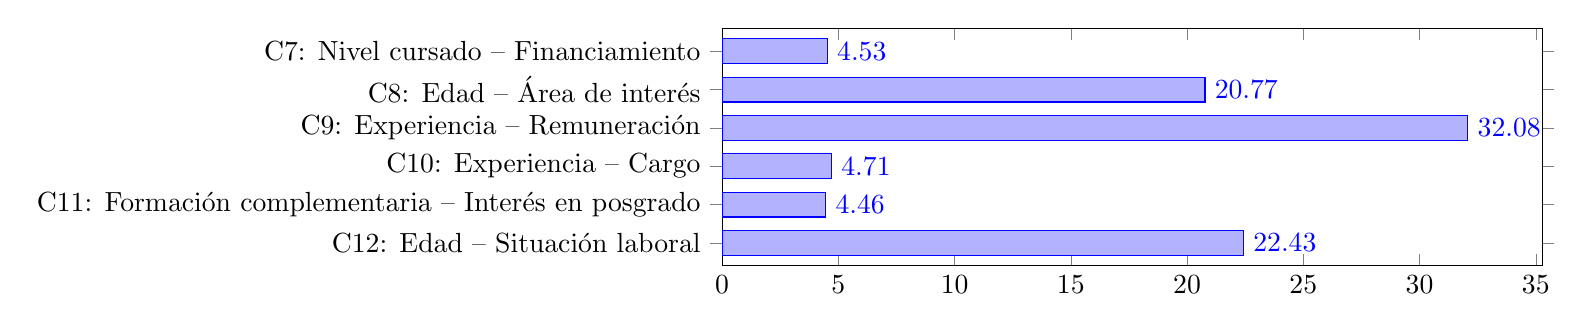
\begin{tikzpicture}
\begin{axis}[
  xbar, bar width=9pt,
  width=12cm, height=4.6cm,
  xmin=0,
  ytick={0,...,5},
  yticklabels={C7: Nivel cursado -- Financiamiento,C8: Edad -- Área de interés,C9: Experiencia -- Remuneración,C10: Experiencia -- Cargo,C11: Formación complementaria -- Interés en posgrado,C12: Edad -- Situación laboral},
  ymin=-0.6, ymax=5.6,
  nodes near coords, y dir=reverse,
  every axis plot/.style={fill=gray!60}
]
\addplot coordinates {(4.53,0) (20.77,1) (32.08,2) (4.71,3) (4.46,4) (22.43,5) };
\end{axis}
\end{tikzpicture}
\end{figure}

El análisis multivariable de la Sección~\ref{sec:resultado-multivariable} complementa esta lista: mientras que estos cruces dicen \emph{si} dos variables están relacionadas, el multivariable describe \emph{cómo} se ve esa relación sobre una tercera variable cuantitativa.

